\section{Challenges of offshore wind turbines installation}
The challenges of installing offshore wind turbines is due to several factors. Firstly, wind turbine are made up of various large and heavy components that are produced in different sites. Secondly, there are various possible installation scenarios depending on infrastructure and transport vessels availabilities. Thirdly, the installation of the offshore wind turbines is strongly influenced by weather conditions.  
Finally, the material process flow can be affected by various disturbances.

\subsection{Wind turbine components}
An offshore wind turbine usually consist of, see Figure \ref{FigureComponents}:

\begin{itemize}
\item A foundation -- that can be of several types, see Figure \ref{FigureFoundations}. Types of foundation will determine the type of equipment required for installation. For instance, a mono pile foundation will require heavy hydraulic hammer works to ram steel pipes with diameters of 4 meters up to 20 meters into the seabed.

\begin{enumerate}
\item[a] -- Mono pile foundations: they can be either concrete or pre-stressed, used for low or mid-level water depths, and having as advantage low levels of noise emission in operation, low maintenance, material availability with large-scale production.
\item[b] -- Tripod foundations: designs tend to rely on technology used by the oil and gas industry. The piles on each end are typically driven into the seabed, used for deeper depths and have not been used on many projects until now.
\item[c] -- Jacket foundations: can be made of a steel framework with pile foundation, used mainly for great level water depths and have the advantages of light weight and high rigidity.
\item[d] -- Gravity foundations: they can be made of restrained steel pile, used mainly for lower level water depths and having the advantage of being a simple and cost-efficient construction for small depths. 
\end{enumerate}

\item Piles -- The piles are used to fix the foundation to the seabed. During this process, a template is used when hammering or vibrating piles into the seabed. Afterwards, the jacket could be lowered to the bottom of the sea, where the spikes fixed at the end of the legs of the jacket fit into the piles.
\item Tower segments -- have the structural role of carrying the top loads to the foundation. They are made from steel sheet rings and stiffeners (longitudinal or circular, used for rigidity purposes) protected against the strong corrosion due to sea water.
\item One nacelle (machine house) -- results from a combination between a steel lattice structure and fiber glass housing. The hydraulic, electrical and electro-mechanic internal components of the nacelle (gearbox, transformers, cooling systems, etc.) are integrated progressively during the construction of the nacelle. It is important to consider that the nacelle is very heavy (125 tons for a 4MW turbine). Together with the rotor, the weight of the nacelle represents a big problem in terms of lifting capacities.
\item One rotor hub -- it corresponds to the mechanical part that joins the 3 blades together with the nacelle.
\item Three blades -- offshore wind turbines blades are made of composite material. At presents wind blades are mainly made of reinforced fiber glass. For very large blades, carbon fibers have been introduced by many manufacturers in order to reduce the structure weight. The size of the blades is increasing proportionally with the increase in power of the wind turbine. For a 3MW wind turbine, the rotor has a weight of around 100 tons and 100 meters diameter.
\end{itemize}

%???? Cable laying ??????

\begin{figure}[!hbp]
\begin{center}
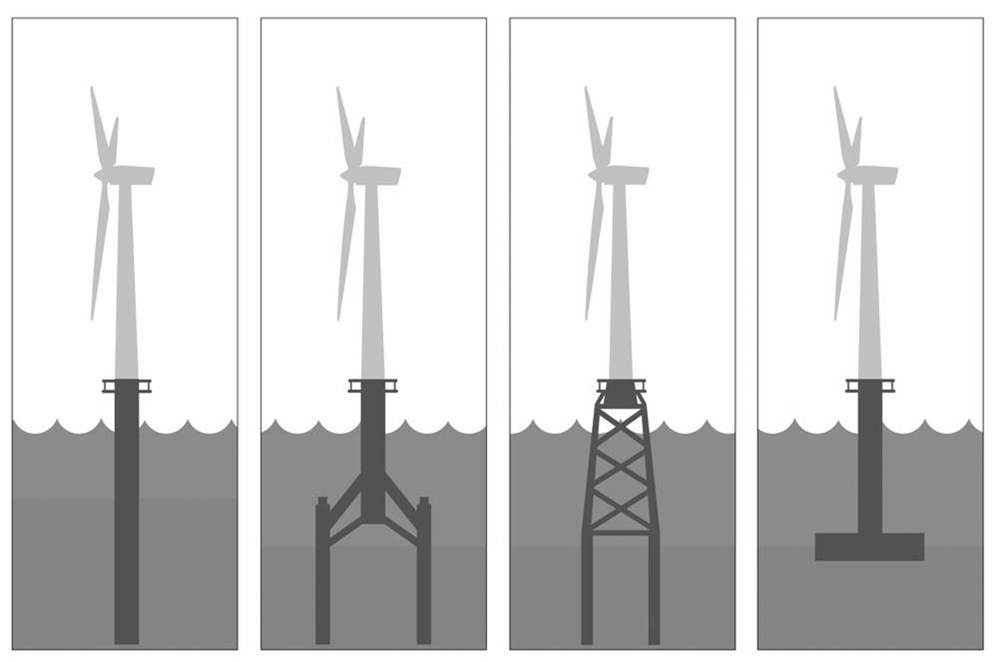
\includegraphics[scale=0.4]{Foundations.jpg} 
\end{center}
\caption{Type of offshore wind turbine foundations -- From left to right, mono pile, Tripod, Jacket and Gravity}
\label{FigureFoundations}
\end{figure}

The size of the newest wind turbines is growing quickly in comparisons with previous generations. The latest generations of wind turbines that will soon be installed at sea have a power of 6 MW, which largely outperform the currently installed offshore wind turbines, whose power does not exceed 5 MW. The current trend is to develop high power machines to increase the energy produced by the OWFs, while reducing the number of machines. The size of the turbines significantly increases the difficulty of construction and the risks during assembly at sea. Moreover, as offshore machines increase in size and weight, more manufacturers will be relocated directly to or in the proximity of the port facilities to ease transportation of machines and delivery of components.

Today, the supply chain for offshore wind turbines relies on processes that already exist in onshore wind industry and offshore structures for the gas and oil sector. In the future, the experience gained from OWFs and the need to produce in series for large scale projects should lead to standardization and important optimization in the supply chain processes.

%All these components are produced in different locations and can be assembled either onshore or offshore.

In this paper, one jacket foundation, four piles, 2 tower segments, one nacelle, one rotor hub and three rotor blades per wind turbine have been considered in the simulation.
